\subsection{Setup and synthetic validation}
\label{subsec:exp-setup}\label{subsec:exp-synthetic}\label{subsec:exp-T-synthetic}

\paragraph{Synthetic validation (details in
Appendix~\ref{app:synthetic}).} Monte Carlo on the hard distribution
$P^\star$ across $T\in\{2,3,4,8\}$, $r\in\{4,8,16\}$,
$d\in\{128,512,2048\}$, isotropic and four heavy-anisotropy spectra
families: the empirical rate slope is $-2.00 \pm 0.01$ ($95\%$
bootstrap CI, $1000$ trials/configuration), matching the predicted
$-2R/\deff$ of Theorem~\ref{thm:general}; the floor
$B^2(1 - \E[\deff]/(Tr))$ is reproduced to four to five digits; and
the ratio of measured distortion to the Theorem~\ref{thm:general}
bound at $c_{\mathrm{TQ}} = 1$ stays $\leq 13$ across all
configurations, constant in $R$ within bootstrap CI. A
dedicated $T$-sweep ($T$ up to $16$) measures the achievability
constant's growth as logarithmic in $T$ (Remark~\ref{rem:tgap}). In the
floor-positive regime, the null-space construction tracks its predicted
exponent $-2r/(r+|A|-1)$ and a random-codebook encoder is strictly
steeper, confirming the open gap of Remark~\ref{rem:sharedv-gap}.

\paragraph{Real-LLM setup.} We calibrate the bound against real LoRA
fine-tunes on four instruction-tuned bases spanning distinct
pretraining recipes and attention designs: Llama-3.1-8B-Instruct (MHA),
Qwen-2.5-7B-Instruct (GQA), Mistral-7B-Instruct-v0.3 (MHA), and
Yi-1.5-9B-Chat (MHA). For each we train $T=4$ adapters (rank $r = 16$
on the $\{q,k,v,o\}$ projections; AdamW, lr $5\times10^{-5}$, $7500$
examples $\times$ $2$ epochs) on GSM8K (math), Alpaca-cleaned
(instruction following), Magicoder-OSS-Instruct (code), and WMT19
en$\to$de (translation); $16$ adapters total, retrained at three
independent seeds. For a merged delta $w$ we measure per-task
\emph{excess} NLL over the task's own adapter,
$\Delta L_t(w) = L_t(\theta_0 + w) - L_t(\theta_0 + \tau_t)$ on
$n = 1000$ held-out examples (nats per response token), and worst-task
distortion $\widehat D(w) = \max_t \Delta L_t(w)$; the shared frozen
base cancels, isolating the cost of merging. CIs are $95\%$ percentile
bootstrap over $10{,}000$ resamples. A second cohort, the
\emph{$T$-scaling pool} (the four tasks plus CodeAlpaca, Dolly, XSum),
underlies \S\ref{subsec:exp-T-scaling}; excesses are not
cross-comparable between cohorts.

\subsection{The regime of real merging: zero floor, $0.10$--$0.22$ nats
of algorithmic slack}
\label{subsec:exp-lora}\label{subsec:exp-multiseed}

Four findings from the $T = 4$ matrix (five baseline methods: TA, TIES,
DARE at density $0.2$, KnOTS, and TVQ at $b \in \{1,\dots,32\}$ bits).
\textbf{(1) Non-vanishing worst-task excess, zero floor.} At the
no-quantization rate, worst-task excess is strictly positive on every
base (TA: Llama $0.218$, Mistral $0.146$, Qwen $0.110$, Yi $0.099$).
Computing $\deff = \rank(\sum_t P_{V_t})$
directly from the trained adapters gives $\deff = Tr = 64$ in
\emph{every} layer of \emph{every} model: the four task subspaces are
linearly independent, the predicted floor is exactly zero, and the
$0.10$--$0.22$ nats gap is method suboptimality, not an unavoidable
cost of merging. Deliberate attempts to break the saturation ($90\%$
shared training data, rank $r = 64$) fail to move it; a mechanical
barrier explains why ($\deff < Tr$ requires $r > d_{\mathrm{in}}/T$,
far outside the practical LoRA range; Appendix~\ref{app:e5}, with a
floor-estimation recipe). \textbf{(2) Merging difficulty tracks
training recipe, not architecture.} The excess orders Llama $>$
Mistral $>$ Qwen $>$ Yi (non-overlapping CIs), cutting across
attention design and unexplained by either hard rank or a soft
participation-ratio overlap statistic. \textbf{(3) Only TIES
separates from the structure-blind cluster.} TIES cuts worst-task
excess by $30$--$88\%$ vs.\ TA ($3$-seed means), concentrated on the
bottleneck task; KnOTS and DARE are statistically indistinguishable
from TA (paired differences $\leq 0.003$ nats), exactly as the
theory predicts at zero subspace overlap, where alignment has nothing
to exploit. \textbf{(4) A universal ``less-is-more'' dip at $b=2$.}
The TVQ rate sweep is non-monotone on every base: $2$-bit quantization
sits $1.7$--$6.0\times$ below the adjacent $b = 4$ point
(non-overlapping CIs), while $b = 1$ and $b \geq 4$ regress to the
$\approx$TA floor; the dip covaries with TIES per-task but is
\emph{not} explained by implicit sparsity (Appendix~\ref{app:b2}).

\paragraph{Seed robustness.} Retraining the matrix at three
independent seeds and running $10{,}000$-resample paired bootstraps on
the five method-pair gaps behind our recommendations leaves \emph{all
$20$ gaps Confident} (largest CI half-width $\pm 0.0044$ nats;
Appendix~\ref{app:multiseed}). The $\deff = Tr$ finding is empirical
(trained subspaces are optimized, not random) but holds in
$100\%$ of layers across four independently pretrained models.

\subsection{The exact encoder fails on real adapters; one ridge term
salvages it}
\label{subsec:exp-rd-encoder}

We instantiate the encoder of Theorem~\ref{thm:achv} with the projector
surrogate $H_t = P_{V_t}$ (top-$r$ right-singular projector of each
task's delta), evaluated at the $b \to \infty$ rate on Llama-3.1-8B at
$T = 4$. \textbf{The exact centroid fails:} worst-task excess $0.340$
($3$-seed mean), \emph{worse} than TA ($0.220$) and more than $2\times$
TIES ($0.154$). The mechanism is spectral: $\bar H$'s non-zero
spectrum is nearly degenerate (median $\approx 2\times 10^{-3}$,
minimum $\approx 10^{-5}$), and the pseudo-inverse divides by these
sliver eigenvalues, amplifying $\|w^\star\|$ to $25$--$94\times$ the
TA norm, far outside the quadratic surrogate's validity region; the
failure is in the surrogate$\to$CE bridge, not in the construction's
surrogate optimality.

\textbf{The salvage.} Replacing $\bar H^{+}$ with
$(\bar H + \lambda I)^{-1}$, the same construction with a numerical
sliver-floor exposed as one hyperparameter, produces a clean U-curve
with minimum at $\lambda^\star = 0.05$: worst-task excess
$\mathbf{0.094}$, $57\%$ below TA and $39\%$ below TIES
(Figure~\ref{fig:salvage}). The sweep, per-task breakdown, and a
Fisher-diagonal sanity check are in Appendix~\ref{app:robustness}. The
salvage generalizes: each base has a well-defined optimum
($\lambda^\star = 0.05$ on Llama, $0.13$ on the other three), and the
\emph{single globally-fixed} $\lambda = 0.13$ (the leave-one-base-out
modal choice) already beats TA and TIES on all four bases
($0.125/0.044/0.010/0.037$).

\begin{figure}[t]
\centering
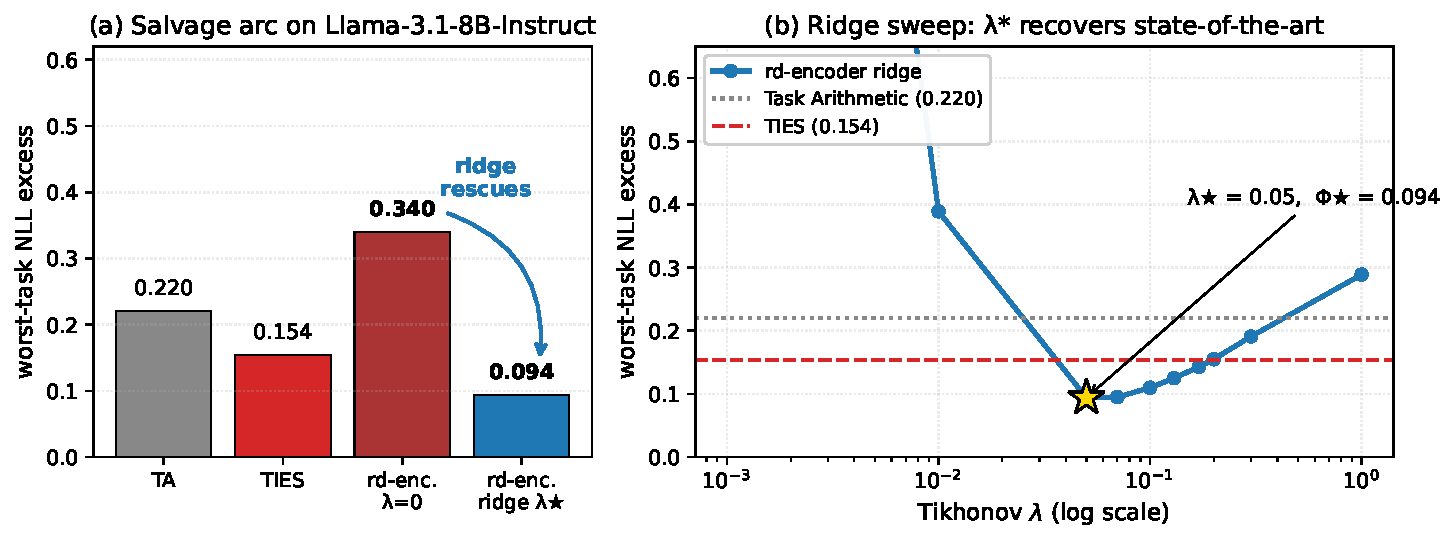
\includegraphics[width=0.85\textwidth]{figures/figure_salvage_arc.pdf}
\caption{\textbf{Salvage arc.} (a) On Llama-3.1-8B-Instruct at $T = 4$,
the exact rd-encoder construction ($\lambda = 0$) collapses to
worst-task excess $0.340$, above TA ($0.220$) and TIES ($0.154$);
Tikhonov regularization at $\lambda^\star = 0.05$ recovers $0.094$,
the lowest figure for this base. (b) rd-encoder ridge sits below both
TA and TIES across the band $[0.03, 0.18]$. All values are $3$-seed
means on matched seed-$1/2/3$ adapters.}
\label{fig:salvage}
\end{figure}

\begin{table}[t]
\centering
\caption{Unified head-to-head: worst-task NLL excess ($T = 4$ matrix)
for ten methods at default hyperparameters. \textsc{rd-encoder ridge}
(base-optimal $\lambda$) is its $3$-seed mean on matched seed-$1/2/3$
adapters; the four added closed-form baselines are seed-$1$ cells
(seed-stable to $\pm 0.01$; Appendix~\ref{app:multiseed}).}
\label{tab:e10-baselines}
\small
\begin{tabular}{lrrrr}
\hline
Method & Llama-3.1 & Mistral-7B & Qwen-2.5 & Yi-1.5 \\
\hline
Task Arithmetic           & $0.213$ & $0.133$ & $0.104$ & $0.099$ \\
TIES                      & $0.147$ & $0.049$ & $0.013$ & $0.045$ \\
DARE                      & $0.213$ & $0.134$ & $0.107$ & $0.101$ \\
KnOTS                     & $0.213$ & $0.132$ & $0.104$ & $0.099$ \\
TVQ ($b{=}2$)             & $0.101$ & $0.054$ & $0.019$ & $0.057$ \\
Fisher-magnitude          & $0.148$ & $0.050$ & $0.014$ & $0.053$ \\
DELLA                     & $0.131$ & $0.052$ & $0.014$ & $0.055$ \\
RegMean (data-free)       & $0.243$ & $0.054$ & $0.034$ & $0.045$ \\
AdaMerging (data-free)    & $0.228$ & $0.113$ & $0.087$ & $0.075$ \\
\textsc{rd-encoder ridge} & $\mathbf{0.094}$ & $\mathbf{0.044}$ & $\mathbf{0.010}$ & $\mathbf{0.037}$ \\
\hline
\end{tabular}
\end{table}

\textbf{Head-to-head and the tuning question.}
Table~\ref{tab:e10-baselines} places rd-encoder ridge in one
seed-consistent comparison with nine baselines, including its closest
structural relative, data-free RegMean~\citep{jin2023regmean}, and
data-free AdaMerging~\citep{adamerging2024}: lowest worst-task excess
on every base at default hyperparameters. Because a swept $\lambda$
against untuned baselines would be an unfair win, we also sweep each
close competitor's key hyperparameter (TIES/DARE density over five
values, RegMean's own ridge $\lambda$ over six decades;
Appendix~\ref{app:robustness}): rd-encoder ridge remains best on
Llama, Mistral, and Qwen against every tuned competitor, but on
saturated Yi-Chat a tuned RegMean edges it ($0.033$ vs.\ $0.037$,
consistent across three matched seeds) and a tuned TIES ties it. We
therefore claim the strongest data-free merge \emph{robustly on the
non-saturated bases} and competitive-but-not-dominant on saturated
Yi, the base where we independently flag NLL excess as an unreliable
proxy (R2). Part of the default-hyperparameter
Llama gap over RegMean ($0.243$) is the same sliver pathology that
breaks our own $\lambda = 0$ construction ($0.340$): RegMean has no
ridge term, which is precisely why the tuned-RegMean control matters.

\subsection{$T$-scaling and the TIES-inversion audit}
\label{subsec:exp-T-scaling}

To test whether the ordering survives beyond $T = 4$, we sweep
$T \in \{2, 4, 7\}$ on three bases (Yi-1.5-9B-Chat,
Llama-3.1-8B-Instruct, and pre-registered Mistral-7B-v0.3) over the
seven-task pool ($162$ merge cells, six methods, identical subset
composition across bases). Figure~\ref{fig:hero} plots the sweep; the
full numbers are in Table~\ref{tab:e6-worst}
(Appendix~\ref{app:tscaling}).

\paragraph{The salvage grows with $T$.} On Llama, rd-encoder ridge is
best at every $T$ with a widening margin (ratio rd-ridge/TA
$0.84 \to 0.68 \to 0.52$); the same strengthening holds on Mistral
($1.38 \to 0.82 \to 0.47$, computed from unrounded excess): rd-ridge
loses narrowly at $T = 2$ but wins outright at $T = 7$. Worst-task
excess follows $a + b\log T$ on all three bases ($R^2 \geq 0.93$ on
$16$ of $18$ fits), the real-data counterpart of the synthetic
$\log T$ prediction, and rd-ridge has the lowest and most
base-invariant slope ($0.070/0.065/0.062$ on Yi/Llama/Mistral vs.\
$0.079$--$0.171$ for the matrix methods).

\paragraph{The TIES inversion, and an audit that predicts it.} On Yi,
TIES becomes the \emph{worst} method at $T = 7$; on Llama and Mistral
it does not. A per-coordinate sign-vote probe on the $T = 7$ cohorts
(CPU-only, a few minutes per cohort) locates the difference not in
vote-split structure but in the \emph{per-task win-share range} $R$:
$0.077$ on Yi vs.\ $0.028$ on Llama (Appendix~\ref{app:tscaling}):
on a saturated base tasks sharing instruction-following structure
dominate the vote, and the code and near-saturated adapters are
systematically outvoted. A perturbation
model of the TIES update (Appendix~\ref{app:sign-election-threshold})
converts this into a threshold: predicted ambiguity window
$R^\star \in [0.025, 0.075]$, with inversion above it and TIES winning
outright below it. Yi ($R = 0.077$, above) inverts; Llama
($R = 0.028$, inside) is ambiguous. We then \textbf{pre-registered} an
out-of-sample test (commit \texttt{3582799} in the supplementary audit
trail, timestamped before the Mistral sweep ran): Mistral-7B, probe
range $R = 0.0326$, inside the window, predicted ambiguous at $T = 7$
under operationalized criteria fixed in advance (``clearly worst'' $=$
last and $> \mathrm{TA} + 0.04$; ``clearly best'' $=$ first by
$> 0.02$). The sweep confirms it: TIES second of six, $0.092$ nats
\emph{below} TA, so neither condition fires. A base-free synthetic
experiment closes the causal loop: a single sign-conflict knob raises
$R$ and the TIES$-$TA gap in lockstep (Pearson $0.998$;
Appendix~\ref{app:sign-election-threshold}). \emph{Caveats, stated
plainly:} the window's constants were fit to the two in-sample points,
``ambiguous'' is the prior-likely outcome for most methods, and the
below-window prediction is untested (no cohort we measured has
$R < 0.028$). We present the threshold as a calibrated heuristic with
one out-of-sample consistency check, not a validated law.

\subsection{Do NLL conclusions hold on task accuracy?}
\label{subsec:exp-downstream-gsm8k}

NLL excess is fast and seed-stable but not what a practitioner
deploys against, so we re-merge the $T = 4$ matrix and evaluate GSM8K
exact-match ($n = 500$, greedy CoT) and HumanEval pass@1 ($n = 164$,
sandboxed) on matched seed-$1/2/3$ adapters ($3$-seed means;
Table~\ref{tab:downstream}); rd-encoder ridge runs at the $\lambda$
chosen on NLL and never sees an accuracy metric.

\begin{table}[t]
\centering
\caption{Downstream accuracy ($3$-seed means). Spearman $\rho$ is
computed across the five matrix baselines between accuracy and $-$NLL
excess: positive $\rho$ means NLL ranking predicts accuracy ranking.
Each cell has $n = 5$ methods and is individually low-powered; the
signal is the across-cell pattern, $7$ of $8$ cells positive.
Falsification tests and per-seed stability in
Appendix~\ref{app:downstream}.}
\label{tab:downstream}
\small
\setlength{\tabcolsep}{5pt}
\begin{tabular}{lrrrrrr|r}
\hline
 & TA & TIES & DARE & KnOTS & TVQ$_2$ & rd-ridge & $\rho$ \\
\hline
\multicolumn{8}{l}{\emph{GSM8K exact-match}} \\
Llama-3.1-8B    & $0.315$ & $0.256$ & $0.317$ & \best{$0.323$} & $0.299$ & \worst{$0.201$} & $-0.60$ \\
Mistral-7B-v0.3 & $0.103$ & $0.409$ & $0.103$ & \worst{$0.097$} & $0.379$ & \best{$0.469$} & $+0.67$ \\
Qwen-2.5-7B     & $0.223$ & $0.706$ & \worst{$0.208$} & $0.218$ & $0.685$ & \best{$0.794$} & $+1.00$ \\
Yi-1.5-9B       & $0.763$ & $0.783$ & \worst{$0.751$} & $0.759$ & $0.769$ & \best{$0.791$} & $+0.90$ \\
\hline
\multicolumn{8}{l}{\emph{HumanEval pass@1}} \\
Llama-3.1-8B    & \worst{$0.055$} & $0.354$ & $0.059$ & $0.057$ & $0.441$ & \best{$0.457$} & $+1.00$ \\
Mistral-7B-v0.3 & $0.053$ & \best{$0.250$} & $0.057$ & \worst{$0.045$} & $0.244$ & $0.191$ & $+0.60$ \\
Qwen-2.5-7B     & $0.016$ & $0.547$ & \worst{$0.014$} & $0.016$ & \best{$0.644$} & $0.606$ & $+0.87$ \\
Yi-1.5-9B       & \worst{$0.061$} & $0.081$ & $0.069$ & $0.069$ & $0.081$ & \best{$0.108$} & $+0.72$ \\
\hline
\end{tabular}
\end{table}

\paragraph{Headline.} The NLL$\to$accuracy correspondence is positive
on $7$ of $8$ base$\times$metric cells, meeting the pre-specified
$\rho \geq 0.7$ threshold on $5$; the single inversion
(Llama-3.1, GSM8K \textsc{em}, $\rho = -0.60$) does not replicate on
HumanEval, and both pre-specified mechanism candidates for it were
falsified (Appendix~\ref{app:downstream}). The methods that minimize NLL excess
(TIES, TVQ$_2$, rd-ridge) also produce far more deployable code merges:
TA/DARE/KnOTS cluster $2$--$40\times$ below them on pass@1.

\paragraph{\textsc{rd-encoder ridge} on accuracy: strong, not a
sweep.} rd-ridge is best of six on \emph{five of eight} cells; its
GSM8K wins on Qwen ($+0.088$ over TIES) and Mistral ($+0.060$) are an
order of magnitude larger than its across-seed SD there. On two of the
three cells it does not lead, Llama-3.1 GSM8K (worst of six,
$0.201$) and Mistral HumanEval (third, $0.191$), it is
\emph{seed-unstable} (across-seed SD $0.074$ and $0.084$ vs.\
$\leq 0.015$ on the cells it wins or ties): the norm-amplifying ridge
construction can push greedy generation into degenerate regions on
particular adapter draws, a fragility invisible to the seed-stable NLL
it was selected on. An earlier draft claimed best-or-tied on all eight
cells from a single-draw evaluation; on matched three-seed means that
claim is \textbf{retracted}. The robust result is the seed-for-seed
NLL worst-task-excess win on all four bases; the deployment reading is
to select by NLL and verify on $\geq 2$ downstream metrics.

\subsection{Practical recommendations}
\label{sec:practical-recommendations}

Five rules distilled from
\S\ref{subsec:exp-lora}--\S\ref{subsec:exp-downstream-gsm8k}
(decision table in Appendix~\ref{app:manifest}).
\textbf{R1: Default to rd-encoder ridge.} Lowest worst-task NLL
excess on every base at $T = 4$, strictly best at $T = 7$ on Llama and
Mistral; without any sweep, the global $\lambda = 0.13$ still beats TA
and TIES on all four bases. The robust
win is on NLL; accuracy is a majority-of-cells result
(\S\ref{subsec:exp-downstream-gsm8k}). \textbf{R2: Audit base saturation before
trusting NLL comparisons.} On heavily chat-tuned bases, compressed
per-task headroom amplifies excess asymmetries that need not track
deployable quality (Yi's near-saturated Alpaca adapter;
Appendix~\ref{app:tscaling}): renormalize by headroom or exclude
near-saturated adapters; a TIES win-share range above $\sim 0.05$ is
the warning signal.
\textbf{R3: If not rd-encoder ridge, use TIES or TVQ-$b{=}2$, not
TA; avoid TIES on saturated bases.} TIES wins $3$ of $4$ bases
at $T = 4$ but inverts on Yi at $T = 7$; the win-share audit of
\S\ref{subsec:exp-T-scaling} predicts the regime.
\textbf{R4: Verify on $\geq 2$ downstream metrics before
deploying.} NLL predicts accuracy on $7$ of $8$ cells, but the
L3-GSM8K cell shows single-metric verification can mislead.
\textbf{R5: Estimate the floor before assuming you are
algorithm-bound.} The recipe of Appendix~\ref{app:e5} computes
$\Phi^\star_{\mathrm{lower}} = B^2(1 - \deff/(Tr))$ from adapter
artifacts in $\lesssim 1$ CPU-minute per task; every cohort we
measured is floor-zero.
